\section{Analytic Geometry}\label{sec:AnalyticGeometry}

In what follows, we use the notation $(x_1,y_1)$ to represent a point in
the $(x,y)$ coordinate system, also called the $(x,y)$-plane.
Previously, we used $(a,b)$ to represent
an open interval. Notation often gets reused and abused in mathematics, 
but thankfully, it is usually clear from the context what we mean.

In the $(x,y)$ coordinate system we normally write the $x$-axis
horizontally, with positive numbers to the right of the origin, and
the $y$-axis vertically, with positive numbers above the origin.  That
is, unless stated otherwise, we take ``rightward'' to be the positive
$x$-direction and ``upward'' to be the positive $y$-direction.  In a
purely mathematical situation, we normally choose the same scale for
the $x$- and $y$-axes.  For example, the line joining the origin to
the point $(a,a)$ makes an angle of 45${}^\circ$ with the $x$-axis
(and also with the $y$-axis).

In applications, often letters other than $x$ and $y$ are used, and
often different scales are chosen in the horizontal and vertical
directions.

\begin{example}{Data Plot}{DataPlot}
	Suppose you drop a coin from a window, and you want to study how 
	its height above the ground changes from second to second.
	It is natural to let the letter $t$ denote the time
	(the number of seconds since the object was released) and to let the
	letter $h$ denote the height.  For each $t$ (say, at one-second
	intervals) you have a corresponding height $h$.  This information can
	be tabulated, and then plotted on the $(t,h)$ coordinate plane, as
	shown in figure~\ref{fig:data plot}.
\end{example}

\figure[!ht]
\vbox{
	$$\begin{array}{|r|ccccc|}
	\hline
	seconds & 0 & 1 & 2 & 3 & 4\\
	\hline
	meters & 80 & 75.1 & 60.4 & 35.9 & 1.6\\
	\hline
	\end{array}$$ 
	
	\centerline{\vbox{\beginpicture
			\normalgraphs
			%\ninepoint
			\setcoordinatesystem units <2truecm,0.5truemm>
			\setplotarea x from 0 to 4.2, y from 0 to 90
			\axis left shiftedto x=0 ticks numbered from 20 to 80 by 20 /
			\axis bottom shiftedto y=0 ticks numbered from 0 to 4 by 1 /
			\put {$t$} [l] <3pt,0pt> at 4.2 0
			\put {$h$} [l] <3pt,0pt> at 0 90
			\setquadratic
			\plot 0 80 1 75.1 2 60.4 3 35.9 4 1.6 /
			\multiput {$\bullet$} at 0 80 1 75.1 2 60.4 3 35.9 4 1.6 /
			\endpicture}}}
\caption{A data plot, height versus time. \label{fig:data plot}}
\endfigure

We use the word ``quadrant'' for each of the four regions into which
the plane is divided by the axes: the first quadrant is where points
have both coordinates positive, or the ``northeast'' portion of the
plot, and the second, third, and fourth quadrants are counted off
counterclockwise, so the second quadrant is the northwest, the third
is the southwest, and the fourth is the southeast.

Suppose we have two points $A$ and $B$ in the $(x,y)$-plane.
We often want to know the change in $x$-coordinate (also called the
``horizontal distance'') in going from $A$ to $B$.  This is often
written $\Delta x$, where the meaning of $\Delta$ (a capital delta in
the Greek alphabet) is ``change in''. Thus, $\Delta x$ can be read as
``change in $x$'' although it usually is read as ``delta $x$''. The
point is that $\Delta x$ denotes a single number, and should not be
interpreted as ``delta times $x$''. Similarly, the ``change in $y$'' is written $\Delta y$
and represents the difference between the $y$-coordinates of the 
two points. It is the vertical distance you have to move in going from $A$ to $B$.

\begin{example}{Change in $x$ and $y$}{ChangeIn}\label{ChangeIn}
	If $A=(2,1)$ and $B=(3,3)$ the change in $x$ is
	$$\Delta x=3-2=1$$
	while the change in $y$ is
	$$\Delta y= 3-1=2.$$
	\vspace{-0.5cm}
\end{example}

The general formulas for the change in $x$ and the change in $y$ 
between a point $(x_1,y_1)$ and a point $(x_2,y_2)$ are:
$$
\Delta x=x_2-x_1,\qquad\qquad\Delta y=y_2-y_1.
$$
Note that either or both of these might be negative.

% Input each subsection
%In what follows, we use the notation $(x_1,y_1)$ to represent a point in
%the $(x,y)$ coordinate system, also called the $(x,y)$-plane.
%Previously, we used $(a,b)$ to represent
%an open interval. Notation often gets reused and abused in mathematics, 
%but thankfully, it is usually clear from the context what we mean.
%
%In the $(x,y)$ coordinate system we normally write the $x$-axis
%horizontally, with positive numbers to the right of the origin, and
%the $y$-axis vertically, with positive numbers above the origin.  That
%is, unless stated otherwise, we take ``rightward'' to be the positive
%$x$-direction and ``upward'' to be the positive $y$-direction.  In a
%purely mathematical situation, we normally choose the same scale for
%the $x$- and $y$-axes.  For example, the line joining the origin to
%the point $(a,a)$ makes an angle of 45${}^\circ$ with the $x$-axis
%(and also with the $y$-axis).
%
%In applications, often letters other than $x$ and $y$ are used, and
%often different scales are chosen in the horizontal and vertical
%directions.  \\
%
%\begin{example}{Data Plot}{DataPlot}
%Suppose you drop a coin from a window, and you want to study how 
%its height above the ground changes from second to second.
%It is natural to let the letter $t$ denote the time
%(the number of seconds since the object was released) and to let the
%letter $h$ denote the height.  For each $t$ (say, at one-second
%intervals) you have a corresponding height $h$.  This information can
%be tabulated, and then plotted on the $(t,h)$ coordinate plane, as
%shown in figure~\ref{fig:data plot}.
%\end{example}
%
%\figure[!ht]
%\vbox{
%$$\begin{array}{|r|ccccc|}
%\hline
%seconds & 0 & 1 & 2 & 3 & 4\\
%\hline
%meters & 80 & 75.1 & 60.4 & 35.9 & 1.6\\
%\hline
%\end{array}$$ 
%
%\centerline{\vbox{\beginpicture
%\normalgraphs
%%\ninepoint
%\setcoordinatesystem units <2truecm,0.5truemm>
%\setplotarea x from 0 to 4.2, y from 0 to 90
%\axis left shiftedto x=0 ticks numbered from 20 to 80 by 20 /
%\axis bottom shiftedto y=0 ticks numbered from 0 to 4 by 1 /
%\put {$t$} [l] <3pt,0pt> at 4.2 0
%\put {$h$} [l] <3pt,0pt> at 0 90
%\setquadratic
%\plot 0 80 1 75.1 2 60.4 3 35.9 4 1.6 /
%\multiput {$\bullet$} at 0 80 1 75.1 2 60.4 3 35.9 4 1.6 /
%\endpicture}}}
%\caption{A data plot, height versus time. \label{fig:data plot}}
%\endfigure
%
%We use the word ``quadrant'' for each of the four regions into which
%the plane is divided by the axes: the first quadrant is where points
%have both coordinates positive, or the ``northeast'' portion of the
%plot, and the second, third, and fourth quadrants are counted off
%counterclockwise, so the second quadrant is the northwest, the third
%is the southwest, and the fourth is the southeast.
%
%Suppose we have two points $A$ and $B$ in the $(x,y)$-plane.
%We often want to know the change in $x$-coordinate (also called the
%``horizontal distance'') in going from $A$ to $B$.  This is often
%written $\Delta x$, where the meaning of $\Delta$ (a capital delta in
%the Greek alphabet) is ``change in''. Thus, $\Delta x$ can be read as
%``change in $x$'' although it usually is read as ``delta $x$''. The
%point is that $\Delta x$ denotes a single number, and should not be
%interpreted as ``delta times $x$''. Similarly, the ``change in $y$'' is written $\Delta y$
%and represents the difference between the $y$-coordinates of the 
%two points. It is the vertical distance you have to move in going from $A$ to $B$. \\
%
%\begin{example}{Change in $x$ and $y$}{ChangeIn}\label{ChangeIn}
%If $A=(2,1)$ and $B=(3,3)$ the change in $x$ is
%$$\Delta x=3-2=1$$
%while the change in $y$ is
%$$\Delta y= 3-1=2.$$
%\vspace{-0.5cm}
%\end{example}
%
%The general formulas for the change in $x$ and the change in $y$ 
%between a point $(x_1,y_1)$ and a point $(x_2,y_2)$ are:
%$$
%\Delta x=x_2-x_1,\qquad\qquad\Delta y=y_2-y_1.
%$$
%Note that either or both of these might be negative.



%%%%%%%%%%%%%%%%%%
\subsection{Lines}\label{sec:lines}
If we have two \ifont{distinct} points $A(x_1,y_1)$ and $B(x_2,y_2)$, then we can draw one
and only one straight line through both points.  By the \dfont{slope} of this line
we mean the ratio of $\Delta y$ to $\Delta x$.  The slope is often denoted by the letter $m$. \\

\begin{formulabox}[Slope Formula]
The slope of the line joining the points $(x_1,y_1)$ and $(x_2,y_2)$ is:
$$m=\frac{\Delta y}{\Delta x}=\frac{y_2-y_1}{x_2-x_1}=\frac{\mbox{rise}}{\mbox{run}}$$
\end{formulabox}

\bigskip

\begin{example}{Slope of a Line Joining Two Points}{SlopeofLine}
The line joining the two points $(1,-2)$ and $(3,5)$ has slope
$\ds m=\frac{5-(-2)}{3-1}=\frac{7}{2}$
%\vspace{-0.8cm}
\end{example}

The most familiar form of the equation of a straight line is:
$$y=mx+b.$$
Here $m$ is the slope of the line: if you increase $x$ by
1, the equation tells you that you have to increase $y$ by $m$; and if
you increase $x$ by $\Delta x$, then $y$ increases by $\Delta
y=m\Delta x$.  The number $b$ is called the \dfont{y-intercept}, because
it is where the line crosses the $y$-axis (when $x=0$).  If you know two points on
a line, the formula $m=(y_2-y_1)/(x_2-x_1)$ gives you the slope.
Once you know a point and the slope, then the $y$-intercept can be
found by substituting the coordinates of either point in the equation:
$y_1=mx_1+b$, i.e., $b=y_1-mx_1$.  Alternatively, one can use the
\dfont{``point-slope'' form} of the equation of a straight line: start with
$(y-y_1)/(x-x_1)=m$ and then multiply to get 
$$(y-y_1)=m(x-x_1),$$ the
point-slope form. Of course, this may be further manipulated to get
$y=mx-mx_1+y_1$, which is essentially the \dfont{``$y=mx+b$'' form}.

It is possible to find the equation of a line between two points directly
from the relation $m=(y-y_1)/(x-x_1)=(y_2-y_1)/(x_2-x_1)$, which says ``the
slope measured between the point $(x_1,y_1)$ and the point $(x_2,y_2)$ is
the same as the slope measured between the point $(x_1,y_1)$ and any other
point $(x,y)$ on the line.''  For example, if we want to find the equation
of the line joining points $A(2,1)$ and $B(3,3)$, we can use
this formula:
$$
m=\frac{y-1}{x-2}=\frac{3-1}{3-2}=2,\qquad\hbox{so~that}\qquad
y-1=2(x-2),\qquad\hbox{i.e.,}\qquad y=2x-3.
$$
Of course, this is really just the point-slope formula, except that we
are not computing $m$ in a separate step. 
We summarize the three common forms of writing a straight line below:\\

\begin{formulabox}[Slope-Intercept Form of a Straight Line]
An equation of a line with slope $m$ and $y\, $-intercept $b$ is:
$$y=mx+b.$$
\end{formulabox}

\bigskip

\begin{formulabox}[Point-Slope Form of a Straight Line]
An equation of a line passing through $(x_1,y_1)$ and having slope $m$ is:
$$y-y_1=m(x-x_1).$$
\end{formulabox}

\bigskip

\begin{formulabox}[General Form (Standard Form) of a Straight Line]
Any line can be written in the form
$$Ax+By+C=0,$$
where $A,B,C$ are constants and $A,B$ are not both $0$.
\end{formulabox}

The slope $m$ of a line in the form $y=mx+b$ tells us the
direction in which the line is pointing.  If $m$ is positive, the line goes
into the 1st quadrant as you go from left to right.   If $m$ is large and
positive, it has a steep incline, while if $m$ is small and positive, 
then the line has a small angle of inclination.  If $m$ is negative, the
line goes into the 4th quadrant as you go from left to right.  If $m$ is
a large negative number (large in absolute value), then the line points
steeply downward. If $m$ is negative but small in absolute value, then it points
only a little downward.

If $m=0$, then the line is horizontal and its equation is simply $y=b$.

All of these possibilities are illustrated below.
%figure~\ref{fig:graphs of lines}.

$$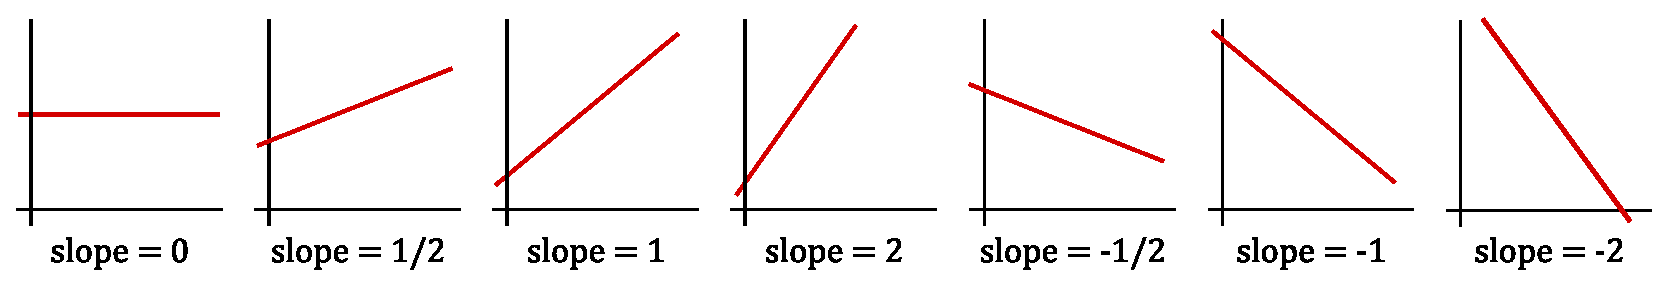
\includegraphics[width=6.4in]{images/slopes}$$

%\figure[!ht]
%\vbox{
%\centerline{\vbox{\beginpicture
%\normalgraphs
%%\sevenpoint
%\setcoordinatesystem units <3truemm,3truemm>
%\setplotarea x from -5 to 5, y from -5 to 5
%\axis left shiftedto x=0 /
%\axis bottom shiftedto y=0 /
%\setlinear
%\plot -1 -5 2.33 5 /
%\linethickness 0.1pt
%\axis left ticks in andacross from -5 to 5 by 1 /
%\axis left ticks in andacross numbered from -4 to 4 by 2 /
%\axis bottom ticks in andacross from -5 to 5 by 1 /
%\axis bottom ticks in andacross numbered from -4 to 4 by 2 /
%\endpicture}\qquad\vbox{\beginpicture
%\normalgraphs
%%\sevenpoint
%\setcoordinatesystem units <3truemm,3truemm>
%\setplotarea x from -5 to 5, y from -5 to 5
%\axis left shiftedto x=0 /
%\axis bottom shiftedto y=0 /
%\setlinear
%\plot -5 1 5 2 /
%\linethickness 0.1pt
%\axis left ticks in andacross from -5 to 5 by 1 /
%\axis left ticks in andacross numbered from -4 to 4 by 2 /
%\axis bottom ticks in andacross from -5 to 5 by 1 /
%\axis bottom ticks in andacross numbered from -4 to 4 by 2 /
%\endpicture}\qquad\vbox{\beginpicture
%\normalgraphs
%%\sevenpoint
%\setcoordinatesystem units <3truemm,3truemm>
%\setplotarea x from -5 to 5, y from -5 to 5
%\axis left shiftedto x=0 /
%\axis bottom shiftedto y=0 /
%\setlinear
%\plot -0.5 5 2 -5 /
%\linethickness 0.1pt
%\axis left ticks in andacross from -5 to 5 by 1 /
%\axis left ticks in andacross numbered from -4 to 4 by 2 /
%\axis bottom ticks in andacross from -5 to 5 by 1 /
%\axis bottom ticks in andacross numbered from -4 to 4 by 2 /
%\endpicture}\qquad\vbox{\beginpicture
%\normalgraphs
%%\sevenpoint
%\setcoordinatesystem units <3truemm,3truemm>
%\setplotarea x from -5 to 5, y from -5 to 5
%\axis left shiftedto x=0 /
%\axis bottom shiftedto y=0 /
%\setlinear
%\plot -5 2 5 1 /
%\linethickness 0.1pt
%\axis left ticks in andacross from -5 to 5 by 1 /
%\axis left ticks in andacross numbered from -4 to 4 by 2 /
%\axis bottom ticks in andacross from -5 to 5 by 1 /
%\axis bottom ticks in andacross numbered from -4 to 4 by 2 /
%\endpicture}}}
%\caption{Lines with slopes 3, $0.1$, $-4$, and $-0.1$.\label{fig:graphs of lines}}
%\endfigure

There is one type of line that cannot be written in the form $y=mx+b$,
namely, vertical lines.  A vertical line has an equation of the form $x=a$.
Sometimes one says that a vertical line has an ``infinite'' slope.

It is often useful to find the $x$-intercept of a line $y=mx+b$.  This is
the $x$-value when $y=0$.  Setting $mx+b$ equal to 0 and solving for
$x$ gives: $x=-b/m$.  \\

\begin{example}{Finding $x$-intercepts}{xintercepts}
To find $x$-intercept of the line $y=2x-3$, we set $y=0$ and solve for $x$:
$$0 = 2x-3\qquad\to\qquad x = \frac{3}{2}.$$
Thus, the line has an $x$-intercept of $3/2$.
\end{example}

It is often necessary to know if two lines are parallel or perpendicular.
Let $m_1$ and $m_2$ be the slopes of the nonvertical lines $L_1$ and $L_2$.
Then:
\begin{itemize}
\item $L_1$ and $L_2$ are \dfont{parallel} if and only if $m_1=m_2$.
\item $L_1$ and $L_2$ are \dfont{perpendicular} if and only if $\ds{m_2=\frac{-1}{m_1}}$.
\end{itemize}
In the case of perpendicular lines, we say their slopes are \ifont{negative reciprocals}. 
Below is a visual representation of a pair of parallel lines and a pair of perpendicular lines.
$$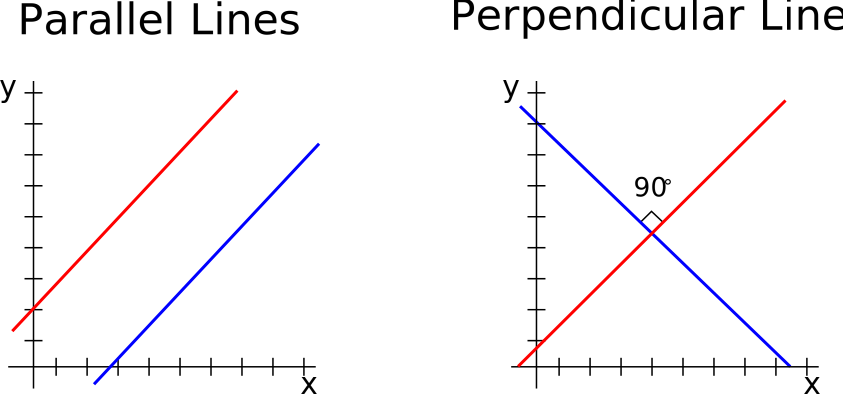
\includegraphics[width=3.7in]{images/lines-1}$$

\begin{example}{Equation of a Line}{EquationLine}
For each part below, find an equation of a line satisfying the requirements:
\begin{enumerate}
\item[(a)] Through the two points $(0,3)$ and $(-2,4)$.
\item[(b)] With slope $7$ and through point $(1,-2)$.
\item[(c)] With slope $2$ and $y$-intercept $4$.
\item[(d)] With $x$-intercept $8$ and $y$-intercept $-3$.
\item[(e)] Through point $(5,3)$ and parallel to the line $2x+4y+2=0$.
\item[(f)] With $y$-intercept $4$ and perpendicular to the line $\ds{y=-\frac{2}{3}x+3}$.
\end{enumerate}
\end{example}

\begin{solution} 
\noindent(a) We use the \ifont{slope formula} on $(x_1,y_1)=(0,3)$ and $(x_2,y_2)=(-2,4)$ to find m:
$$m=\frac{(4)-(3)}{(-2)-(0)}=\frac{1}{-2}=-\frac{1}{2}.$$
Now using the \ifont{point-slope formula} we get an equation to be:
$$y-3=-\frac{1}{2}\left(x-0\right)\quad\to\quad y=-\frac{1}{2}x+3.$$

\noindent(b) Using the \ifont{point-slope formula} with $m=7$ and $(x_1,y_1)=(1,-2)$ gives:
$$y-(-2)=7(x-1)\quad\to\quad y = 7x-9.$$

\noindent(c) Using the \ifont{slope-intercept formula} with $m=2$ and $b=4$ we get $y=2x+4$.

\noindent(d) Note that the intercepts give us two points: $(x_1,y_1)=(8,0)$ and $(x_2,y_2)=(0,-3)$.
Now follow the steps in part (a):
$$m=\frac{-3-0}{0-8}=\frac{3}{8}$$
Using the \ifont{point-slope formula} we get an equation to be:
$$y-(-3)=\frac{3}{8}\left(x-0\right)\quad\to\quad y=\frac{3}{8}x-3$$

\noindent(e)  The line $2x+4y+2=0$ can be written as:
$$4y = -2x - 2 \quad\to\quad y=-\frac{1}{2}x-\frac{1}{2}$$
This line has slope $-1/2$.
Since our line is \ifont{parallel} to it, we have $m=-1/2$.
Now we have a point $(x_1,y_1)=(5,3)$ and slope $m=-1/2$, thus, the \ifont{point-slope formula} gives:
$$y-3=-\frac{1}{2}\left(x-5\right).$$

\noindent(f) The line $\ds{y=-\frac{2}{3}x+3}$ has slope $m=-2/3$.
Since our line is perpendicular to it, the slope of our line is the \ifont{negative reciprocal}, hence, $m=3/2$.
Now we have $b=4$ and $m=3/2$, thus by the \ifont{slope-intercept formula}, an equation of the line is
$$y=\frac{3}{2}x+4.$$
\vspace{-0.5cm}
\end{solution}


\begin{example}{Parallel and Perpendicular Lines}{ParallelPerpendicularLines}
Are the two lines $7x+2y+3=0$ and $6x-4y+2=0$ perpendicular? Are they parallel? If they are not parallel, what is their point of intersection?
\end{example}

\begin{solution} 
The first line $L_{1}$ re-expressed in slope-intercept form is:
$$7x+2y+3=0\quad\to\quad 2y=-7x-3\quad\to\quad y=-\frac{7}{2}x-\frac{3}{2}.$$
It has slope $m_1=-7/2$.
The second line $L_{2}$ in slope-intercept form is:
$$6x-4y+2=0\quad\to\quad -4y=-6x-2\quad\to\quad y=\frac{3}{2}x+\frac{1}{2}.$$
It has slope $m_2=3/2$. Since $m_1\neq m_2$ the lines are not parallel. The lines are also not perpendicular since $m_1\cdot m_2\neq -1$ (they are not negative reciprocals). Therefore, the lines must intersect.\\
We find points of intersection by setting the $y$ -values of $L_{1} = L_{2}$, and then solve for $x$.

\begin{minipage}{0.6\textwidth}
	In particular, we have
	
	$$\begin{array}{rcl}
	L_{1} & = & L_{2} \\
	\ds{-\frac{7}{2}x-\frac{3}{2}} & = & \ds{\frac{3}{2}x+\frac{1}{2}} \\
	\end{array} $$
	
Solving for $x$ gives $x=-2/5$. \\

Then substituting this 
into either $L_{1}$ or $L_{2}$ \\
gives $y=-1/10$.\\
 
Therefore, the lines intersect at the point $(-2/5,-1/10)$.

\vspace{2cm}
\end{minipage}
\begin{minipage}{0.35\textwidth}
	
\vspace{3mm}	
\hspace{3mm}\includegraphics[width=2.2in]{images/ExampleLines}
\end{minipage}
\end{solution}



\subsection{Distance between Two Points and Midpoints}\label{sec:DistanceAndMidpoints}
Given two points $(x_1,y_1)$ and $(x_2,y_2)$, recall that their
horizontal distance from one another is $\Delta x=x_2-x_1$ and their
vertical distance from one another is $\Delta y=y_2-y_1$. Actually,
the word ``distance'' normally denotes ``positive distance''. $\Delta
x$ and $\Delta y$ are {\it signed\/} distances, but this is clear from
context. The (positive) distance from one point to the other
is the length of the hypotenuse of a right triangle with legs $|\Delta
x|$ and $|\Delta y|$, as shown in figure~\ref{fig:distance between
points}.  The Pythagorean Theorem states that the distance between
the two points is the square root of the sum of the squares of the
horizontal and vertical sides:

\figure[!ht]
\centerline{\vbox{\beginpicture
\normalgraphs
%\ninepoint
\setcoordinatesystem units <0.5truein,0.5truein>
\setplotarea x from 0 to 3, y from 0 to 2
\putrule from 0 0 to 3 0
\putrule from 3 0 to 3 2
\plot 0 0 3 2 /
\put {$(x_1,y_1)$} [r] <-5pt,0pt> at 0 0
\put {$(x_2,y_2)$} [l] <5pt,0pt> at 3 2
\put {$\Delta x$} [t] <0pt,-5pt> at 1.5 0
\put {$\Delta y$} [l] <5pt,0pt> at 3 1
\endpicture}}
\caption{Distance between two points (here, $\Delta x$ and $\Delta y$ are positive). \label{fig:distance between points}}
\endfigure

\begin{formulabox}[Distance Formula]
The distance between points $(x_1,y_1)$ and $(x_2,y_2)$ is
$$\hbox{distance}=\sqrt{(\Delta x)^2+(\Delta y)^2}=\sqrt{(x_2-x_1)^2+ (y_2-y_1)^2}.$$
\end{formulabox}

\bigskip

\begin{example}{Distance Between Two Points}{DistanceExample}
The distance, $d$, between points $A(2,1)$ and $B(3,3)$ is 
$$d=\sqrt{(3-2)^2+(3-1)^2}=\sqrt{5}.$$
\vspace{-1cm}
\end{example}

As a special case of the distance formula, suppose we want to know the
distance of a point $(x,y)$ to the origin.  According to the distance
formula, this is $$\sqrt{(x-0)^2+(y-0)^2}=\sqrt{x^2+y^2}.$$
A point $(x,y)$ is at a distance $r$ from the origin if and only if
$\sqrt{x^2+y^2}=r$, or, if we square both sides: $x^2+y^2=r^2$.  As illustrated
in the next section, this is the equation of the circle of radius, $r$, centered at the origin.

Furthermore, given two points we can determine the \dfont{midpoint} of the line segment joining the two points.\\

\begin{formulabox}[Midpoint Formula]
The midpoint of the line segment joining two points $(x_1,y_1)$ and 
$(x_2,y_2)$ is the point with coordinates:
$$\hbox{midpoint}=\left(\frac{x_1+x_2}{2},\frac{y_1+y_2}{2}\right).$$
\end{formulabox}

\bigskip

\begin{example}{Midpoint of a Line Segment}{Midpoint}
Find the midpoint of the line segment joining the given points: $(1,0)$ and $(5,-2)$.
\end{example}

\begin{solution} 
Using the \ifont{midpoint formula} on $(x_1,y_1)=(1,0)$ and $(x_2,y_2)=(5,-2)$ we get:
$$\left(\frac{(1)+(5)}{2},\frac{(0)+(-2)}{2}\right)=(3,-1).$$
Thus, the midpoint of the line segment occurs at $(3,-1)$.
\end{solution}


\subsection{Conics}\label{sec:Conics}

In this section we review equations of parabolas, circles, ellipses and hyperbolas.
We will give the equations of various conics in \dfont{standard form} along with a sketch.
A useful mnemonic is the following.\\

\begin{formulabox}[Mnemonic]
In each conic formula presented, the terms `$x-h$' and `$y-k$' will always appear. 
The point $(h,k)$ will alway represent either the centre or vertex of the particular conic.
\end{formulabox}

%%%%%%%%%%%%%%%%%%%%%%%%%%%%%%%%%%%%%%%%%%%%%%%%%%%%%%%%%%%
%\subsubsection{Parabolas, circles, ellipses and hyperbolas}

\bigskip\noindent
\dfont{Vertical Parabola:} The equation of a vertical parabola is:
$$y-k=a(x-h)^2$$
$$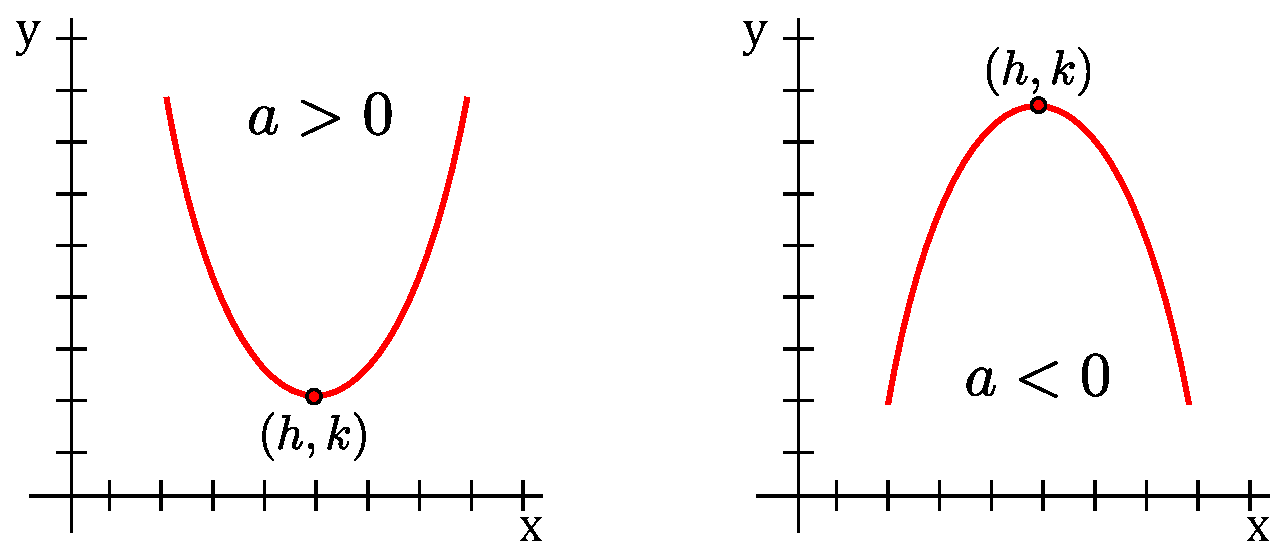
\includegraphics[width=85mm]{images/conics1}$$
\begin{multicols}{2}
\begin{itemize}
	\item $(h,k)$ is the \ifont{vertex} of the parabola.
	\item $a$ is the vertical \ifont{stretch factor}. 
	\item If $a>0$, the parabola opens \ifont{upward}.
	\item If $a<0$, the parabola opens \ifont{downward}.
\end{itemize}
\end{multicols}

\bigskip\noindent
\dfont{Horizontal Parabola:} The equation of a horizontal parabola is:
$$x-h=a(y-k)^2$$
$$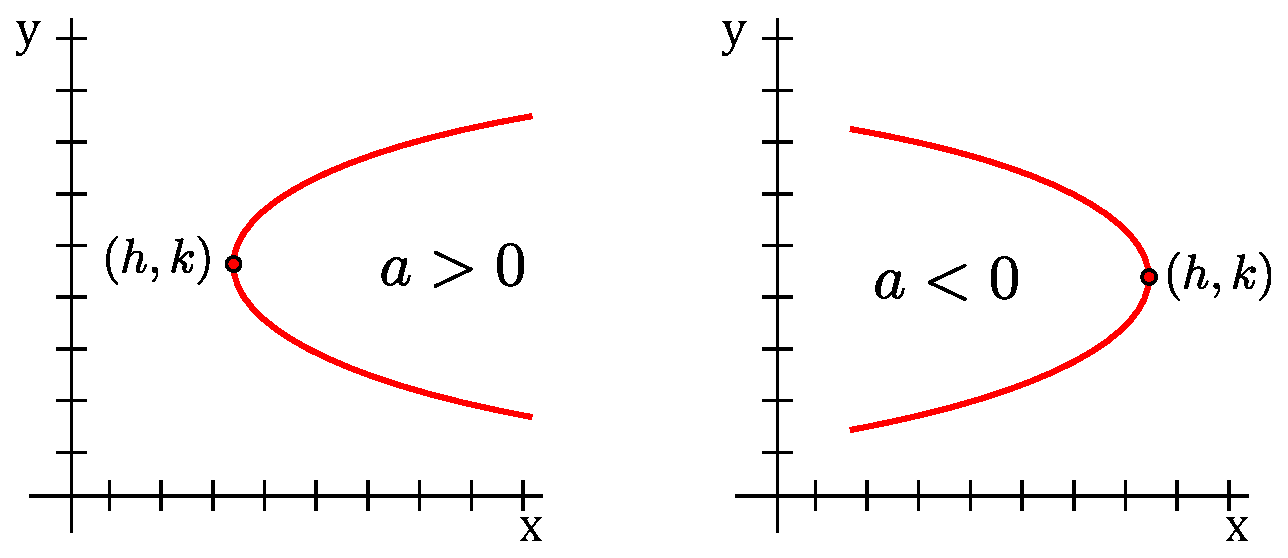
\includegraphics[width=85mm]{images/conics2}$$
\begin{multicols}{2}
\begin{itemize}
	\item $(h,k)$ is the \ifont{vertex} of the parabola.
	\item $a$ is the horizontal \ifont{stretch factor}. 
	\item If $a>0$, the parabola opens \ifont{right}.
	\item If $a<0$, the parabola opens \ifont{left}.
\end{itemize}
\end{multicols} 

\bigskip\noindent
\dfont{Circle:} The equation of a circle is:
$$(x-h)^2+(y-k)^2=r^2$$
$$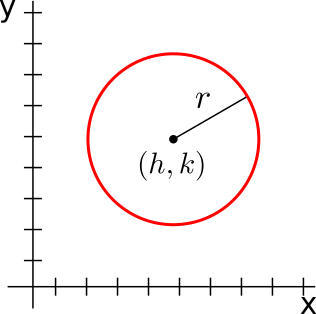
\includegraphics[width=40mm]{images/conics3}$$
\begin{multicols}{2}
\begin{itemize}
	\item $(h,k)$ is the \ifont{centre} of the circle.
	\item  $r$ is the \ifont{radius} of the circle.
\end{itemize}
\end{multicols}

\bigskip\noindent
\dfont{Ellipse:} The equation of an ellipse is:
$$\frac{(x-h)^2}{a^2}+\frac{(y-k)^2}{b^2}=1$$
$$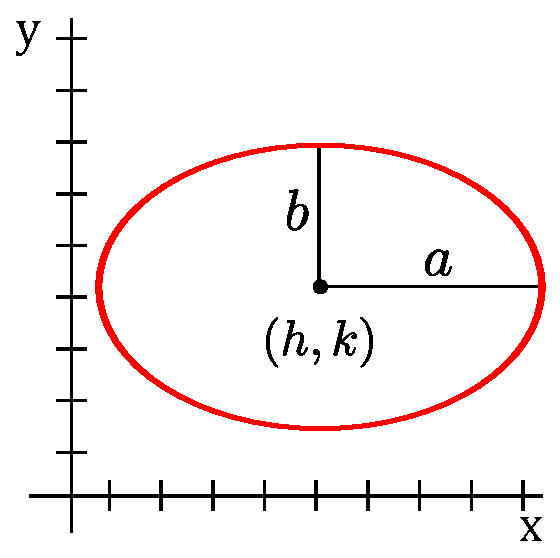
\includegraphics[width=40mm]{images/conics4}$$
\begin{itemize}
	\item $(h,k)$ is the \ifont{centre} of the ellipse.
	\item $a$ is the \ifont{horizontal distance} from the centre to the edge of the ellipse.
	\item $b$ is the \ifont{vertical distance} from the centre to the edge of the ellipse.
\end{itemize}

\bigskip\noindent
\dfont{Horizontal Hyperbola:} The equation of a horizontal hyperbola is:
$$\frac{(x-h)^2}{a^2}-\frac{(y-k)^2}{b^2}=1$$
%$$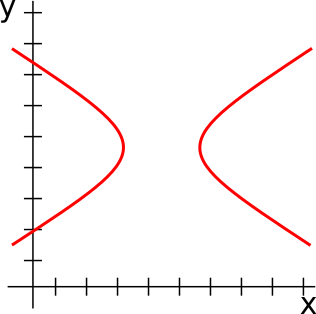
\includegraphics[width=40mm]{images/conics5}$$
\begin{multicols}{2}
\begin{itemize}
	\item $(h,k)$ is the \ifont{centre} of the hyperbola.
	\item $a,b$ are the \ifont{reference box} values. The box has a centre of $(h,k)$.
	\item $a$ is the \ifont{horizontal distance} from the centre to the edge of the box.
	\item $b$ is the \ifont{vertical  distance} from the centre to the edge of the box.
\end{itemize}
\end{multicols}
Given the equation of a horizontal hyperbola, one may sketch it by first placing a dot at 
the point $(h,k)$. Then draw a box around $(h,k)$ with horizontal distance $a$ and vertical distance $b$ to the edge of the box. Then draw dotted lines (called the \dfont{asymptotes} of the hyperbola) through the corners of the box. Finally, sketch the hyperbola in a horizontal direction as illustrated below.
$$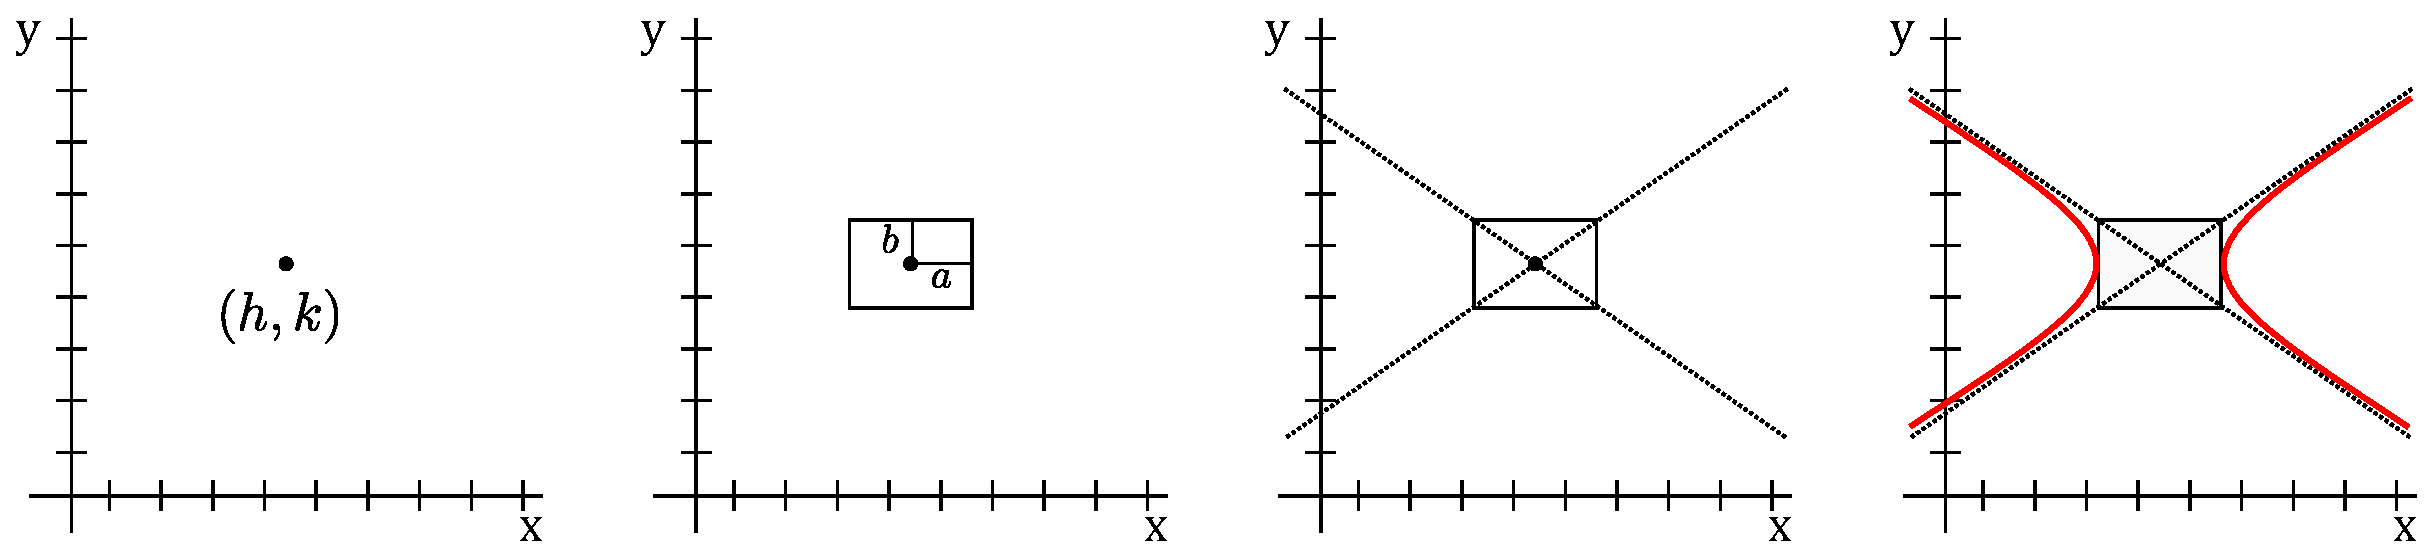
\includegraphics[width=150mm]{images/conics6}$$

\bigskip\noindent
\dfont{Vertical Hyperbola:} The equation of a vertical hyperbola is:
$$\frac{(x-h)^2}{a^2}-\frac{(y-k)^2}{b^2}=-1$$
%$$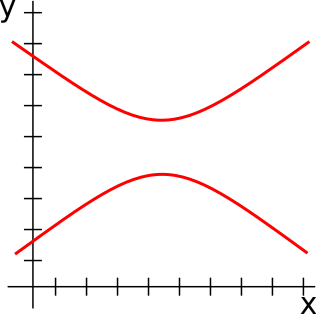
\includegraphics[width=40mm]{images/conics7}$$
\begin{multicols}{2}
\begin{itemize}
	\item $(h,k)$ is the \ifont{centre} of the hyperbola.
	\item $a,b$ are the \ifont{reference box} values. The box has a centre of $(h,k)$.
	\item $a$ is the \ifont{horizontal distance} from the centre to the edge of the box.
	\item $b$ is the \ifont{vertical  distance} from the centre to the edge of the box.
\end{itemize}
\end{multicols}
Given the equation of a vertical hyperbola, one may sketch it by following the same steps as with a horizontal hyperbola, but sketching the hyperbola going in a vertical direction.
$$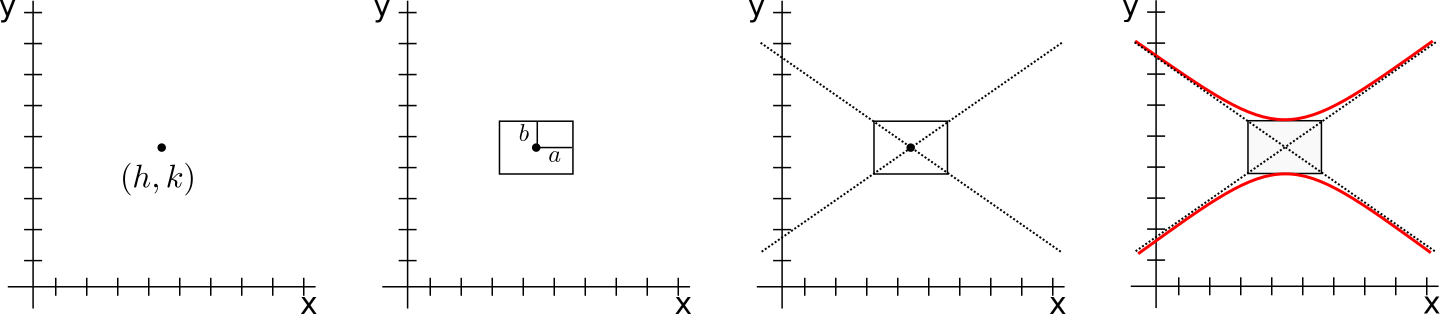
\includegraphics[width=150mm]{images/conics8}$$

\begin{formulabox}[Determining the Type of Conic]
An equation of the form
$$Ax^2+Bxy+Cy^2+Dx+Ey+F=0$$
gives rise to a graph that can be generated by performing a conic section (parabolas, circles, ellipses, hyperbolas).
Note that the $Bxy$ term involves conic rotation. The $Dx$, $Ex$, and $F$ terms affect the vertex and centre.
For simplicity, we will omit the $Bxy$ term.
To determine the type of graph we focus our analysis on the values of $A$ and $C$.
\begin{itemize}\setlength{\itemsep}{0 in}
	\item If $A=C$, the graph is a \ifont{circle}.
	\item If $AC>0$ (and $A\neq C$), the graph is an \ifont{ellipse}.
	\item If $AC=0$, the graph is a \ifont{parabola}.
	\item If $AC<0$, the graph is a \ifont{hyperbola}.
\end{itemize}
\end{formulabox}

%\subsubsection{Completing the square}
%The technique of \dfont{completing the square} allows us to determine the center of a circle/ellipse or the vertex of a parabola.
%It is also an important technique used for other purposes (for example, to derive the quadratic formula you can start by completing the square in $ax^2+bx+c=0$, $a\neq 0$).
%
%The main idea behind completing the square is to turn:
%$$ ax^2 + bx + c$$
%into
%$$a(x - h)^2 + k.$$
%One way to complete the square is to use the following formula:
%$$ax^2+bx+c=a\left(x+\frac{b}{2a}\right)^2-\frac{b^2}{4a^2}+c.$$
%But this formula is a bit complicated, so some students prefer following the steps outlined in the next example.
%
%\begin{example}{Completing the Square}{CompletingSquare}
%Solve $2x^2+12x-32=0$ by completing the square.
%\end{example}
%
%\begin{solution}
%In this instance, we will \ifont{not} divide by $2$ first (usually you would) in order to demonstrate what you should do when the `$a$' value is not $1$.
%
%\bigskip
%
%\begin{tabular}{rl}
%$2x^2+12x-32=0$ & Start with original equation.\\
%\\
%$2x^2+12x=32$ & Move the number over to the other side.\\
%\\
%$2(x^2+6x)=32$ & Factor out the $a$ from the $ax^2+bx$ expression.\\
%\\
%$6~~\to~~\frac{6}{2}=3~~\to~~3^2=\dfont{9}$ & Take the number in front of $x$, \\
%	&  \dfont{divide by $2$}, \\
%	&  then \dfont{square} it.\\
%\\
%$\ifont{2}(x^2+6x+\dfont{9})=32+\ifont{2}\cdot\dfont{9}$ & Add the result to both sides, \\
%	&  taking $a=2$ into account.\\
%\\
%$2(x+3)^2=50$ & Factor the resulting perfect square trinomial.\\
%\\
%~ & \ifont{You have now completed the square!}\\
%\\
%$(x+3)^2=25~~\to~~x=2 \mbox{ or } x=-8$ & To solve for $x$, simply divide by $a=2$ \\
%	& and take square roots.\\
%\end{tabular}
%\end{solution}

\begin{example}{Center and Radius of a Circle}{CenterRadius}
Find the centre and radius of the circle $y^2 + x^2 - 12x + 8y + 43 = 0$.
\end{example}

\begin{solution} 
We need to complete the square twice, once for the $x$ terms and once for the $y$ terms.
We'll do both at the same time.
First let's collect the terms with $x$ together, the terms with $y$ together, and move the number to the other side.
%$$y^2 + x^2 - 12x + 8y + 43 = 0$$
$$(x^2-12x)+(y^2+8y)=-43$$
We add $36$ to both sides for the $x$ term ($-12\to \frac{-12}{2}=-6\to (-6)^2=36$), and $16$ to both sides for the $y$ term ($8\to \frac{8}{2}=4\to (4)^2=16$):
$$(x^2-12x+36)+(y^2+8y+16)=-43+36+16$$
Factoring gives:
$$(x-6)^2+(y+4)^2=3^2.$$
Therefore, the centre of the circle is $(6,-4)$ and the radius is $3$.
\end{solution} 

\begin{example}{Type of Conic}{TypeConic}
What type of conic is $4x^2-y^2-8x+8=0$?
Put it in standard form.
\end{example}

\begin{solution} 
Here we have $A=4$ and $C=-1$.
Since $AC<0$, the conic is a hyperbola.
Let us complete the square for the $x$ and $y$ terms.
First let's collect the terms with $x$ together, the terms with $y$ together, and move the number to the other side.
$$(4x^2-8x)-y^2=-8$$
Now we factor out $4$ from the $x$ terms.
$$4(x^2-2x)-y^2=-8$$
Notice that we don't need to complete the square for the $y$ terms (it is already completed!). To complete the square for the $x$ terms we add \dfont{1} ($-2\to\frac{-2}{2}=-1\to(-1)^2=1$), taking into consideration that the $a$ value is $4$:
$$\ifont{4}(x^2-2x+\dfont{1})-y^2=-8+\ifont{4}\cdot\dfont{1}$$
Factoring gives:
$$4(x-1)^2-y^2=-4$$
A hyperbola in standard form has $\pm1$ on the right side and a positive $x^2$ on the left side, thus, we must divide by $4$:
$$(x-1)^2-\frac{y^2}{4}=-1$$
Now we can see that the equation represents a vertical hyperbola with centre $(1,0)$ (and with $a$ value $\sqrt{1}=1$, and $b$ value $\sqrt{4}=2$).
\end{solution} 




\begin{example}{Equation of Parabola}{EquationParabola}\label{EquationParabola}
Find an equation of the parabola with vertex $(1,-1)$ that passes through the points $(-4, 24)$ and $(7, 35)$.
\end{example}

\begin{solution} 
We first need to determine if it is a vertical parabola or horizontal parabola.
See figure \ref{fig:EquationParabola} for a sketch of the three points $(1,-1)$, $(-4, 24)$ and $(7, 35)$ in the $xy$-plane.
\figure[!ht]
$$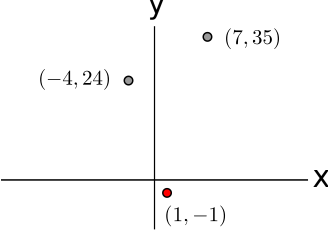
\includegraphics[width=60mm]{images/conics9}$$
\caption{Figure for Example \ref{EquationParabola}\label{fig:EquationParabola}}
\endfigure
Note that the vertex is $(1,-1)$.
Given the location of the vertex, the parabola cannot open downwards.
It also cannot open left or right (because the vertex is between the other two points - if it were to open to the right, every other point would need to be to the right of the vertex; if it were to open to the left, every other point would need to be to the left of the vertex).
Therefore, the parabola must open upwards and it is a vertical parabola.
It has an equation of
$$y-k=a(x-h)^2.$$
As the vertex is $(h,k)=(1,-1)$ we have:
$$y-(-1)=a(x-1)^2$$
To determine $a$, we substitute one of the points into the equation and solve.
Let us substitute the point $(x,y)=(-4,24)$ into the equation:
$$24-(-1)=a(-4-1)^2\quad\to\quad 25=25a\quad\to\quad a=1.$$
Therefore, the equation of the parabola is:
$$y+1=(x-1)^2.$$
Note that if we substituted $(7,35)$ into the equation instead, we would also get $a=1$.
\end{solution}



		

%%%%%%%%%%%%%%%%%%%%%%%%%%%%%%%%%%%%%%%%%%%%%%%%%%%
\Opensolutionfile{solutions}[ex]
\section*{Exercises for \ref{sec:AnalyticGeometry}}

\begin{enumialphparenastyle}

%%%%%%%%%%
\begin{ex}
Find the equation of the line in the form $y=mx+b$:
\begin{enumerate}
	\item	through $(1,1)$ and $(-5, -3)$
	\item	through $(-1,2)$ with slope $-2$
	\item	through $(-1,1)$ and $(5, -3)$
	\item	through $(2,5)$ and parallel to the line $3x+9y+6=0$
	\item	with $x$-intercept 5 and perpendicular to the line $y=2x+4$
\end{enumerate}
\begin{sol}
\begin{enumerate}
	\item	$(2/3)x+(1/3)$
	\item	$y=-2x$
	\item	$y=(-2/3)x+(1/3)$
	\item	$y=-x/3+17/3$
	\item	$y=-1/2x+5/2$
\end{enumerate}
\end{sol}
\end{ex}

%%%%%%%%%%
\begin{ex}
Change the following equations to the form $y=mx+b$, graph the
line, and find the $y$-intercept and $x$-intercept.
\begin{enumerate}
	\item	$y-2x=2$
	\item	$x+y=6$
	\item	$x=2y-1$
	\item	$3=2y$
	\item	$2x+3y+6=0$
\end{enumerate}
\begin{sol}
\begin{enumerate}
	\item	$y=2x+2$, $2$, $-1$
	\item	$y=-x+6$, $6$, $6$
	\item	$y=x/2+1/2$, $1/2$, $-1$
	\item	$y=3/2$, $y$-intercept: $3/2$, no $x$-intercept
	\item	$y=(-2/3)x-2$, $-2$, $-3$
\end{enumerate}
\end{sol}
\end{ex}
 
%%%%%%%%%%
\begin{ex}
Determine whether the lines $3x+6y=7$ and $2x+4y=5$ are parallel.
\begin{sol}
Yes, the lines are parallel as they have the same slope of $-1/2$
\end{sol}
\end{ex}

%%%%%%%%%%
\begin{ex}
Suppose a triangle in the $(x,y)$-plane has vertices $(-1,0)$,
$(1,0)$ and $(0,2)$.  Find the equations of the three lines that lie along
 the sides of the triangle in $y=mx+b$ form.
\begin{sol}
$y=0$, $y=-2x+2$, $y=2x+2$
\end{sol}
\end{ex}

%%%%%%%%%%
\begin{ex}
Let $x$ stand for temperature in degrees Celsius (centigrade), and let
$y$ stand for temperature in degrees Fahrenheit.  A temperature of $0^\circ$C
corresponds to $32^\circ$F, and a temperature of
$100^\circ$C corresponds to $212^\circ$F.  Find the
equation of the line that relates temperature Fahrenheit $y$ to
temperature Celsius $x$ in the form $y=mx+b$.  
Graph the line, and find the point at which this line intersects $y=x$.
What is the practical meaning of this point?
\begin{sol}
$y=(9/5)x+32$, $(-40,-40)$
\end{sol}
\end{ex}

%%%%%%%%%%
\begin{ex}
A car rental firm has the following charges for a certain type of car:
\$25 per day with 100 free miles included, \$0.15 per mile for more than
100 miles.  Suppose you want to rent a car for one day, and you know you'll
use it for more than 100 miles.  What is the equation relating the cost
$y$ to the number of miles $x$ that you drive the car?
\begin{sol}
$y=0.15x+10$
\end{sol}
\end{ex}

%%%%%%%%%%
\begin{ex}
A photocopy store advertises the following prices: 5c~per
copy for the first 20 copies, 4c~per copy for the 21st through
100th copy, and 3c~per copy after the 100th copy.  Let $x$ be the
number of copies, and let $y$ be the total cost of photocopying.  (a)
Graph the cost as $x$ goes from 0 to 200 copies.  (b) Find the
equation in the form $y=mx+b$ that tells you the cost of making $x$
copies when $x$ is more than 100.
\begin{sol}
$0.03x+1.2$
\end{sol}
\end{ex}

%%%%%%%%%%
\begin{ex}
Market research tells you that if you set the price of an item at
\$1.50, you will be able to sell 5000 items; and for every 10 cents you
lower the price below \$1.50 you will be able to sell another 1000 items.
Let $x$ be the number of items you can sell, and let $P$ be the price of
an item.  (a)~Express $P$ linearly in terms of $x$, in other words,
express $P$ in the form $P=mx+b$.  (b)~Express $x$
linearly in terms of $P$.
\begin{sol}
(a) $P=-0.0001x+2$\\
(b) $x=-10000P+20000$
\end{sol}
\end{ex}

%%%%%%%%%%
\begin{ex}
An instructor gives a 100-point final exam, and decides that a score
90 or above will be a grade of 4.0, a score of 40 or below will be a grade
of 0.0, and between 40 and 90 the grading will be linear.  Let $x$ be
the exam score, and let $y$ be the corresponding grade.  Find a formula
of the form $y=mx+b$ which applies to scores $x$ between 40 and 90.
\begin{sol}
$(2/25)x-(16/5)$
\end{sol}
\end{ex}

%%%%%%%%%%
\begin{ex}
Find the distance between the pairs of points:
\begin{enumerate}
	\item	$(-1,1)$ and $(1,1)$.
	\item	$(5,3)$ and $(-7,-2)$.
	\item	$(1,1)$ and the origin.
\end{enumerate}
\begin{sol}
\begin{enumerate}
	\item	$2$
	\item	$\sqrt{2}$
	\item	$\sqrt{2}$
\end{enumerate}
\end{sol}
\end{ex}

%%%%%%%%%%
\begin{ex}
Find the midpoint of the line segment joining the point $(20,-10)$ to the origin.
\end{ex}

%%%%%%%%%%
\begin{ex}
Find the equation of the circle of radius 3 centered at:
\begin{multicols}{2}
\begin{enumerate}
	\item	$(0,0)$
	\item	$(5,6)$
	\item	$(-5,-6)$
	\item	$(0,3)$
	\item	$(0,-3)$
	\item	$(3,0)$
\end{enumerate}
\end{multicols}
\begin{sol}
\begin{enumerate}
	\item	$x^2+y^2=9$
	\item	$(x-5)^2+(y-6)^2=9$
	\item	$(x+5)^2+(y+6)^2=9$
\end{enumerate}
\end{sol}
\end{ex}

%%%%%%%%%%
\begin{ex}
For each pair of points $A(x_1,y_1)$ and $B(x_2,y_2)$ find an equation of
the circle with center at $A$ that goes through $B$.
\begin{multicols}{2}
\begin{enumerate}
	\item	$A(2,0)$, $B(4,3)$
	\item	$A(-2,3)$, $B(4,3)$
\end{enumerate}
\end{multicols}
\end{ex}

%%%%%%%%%%
\begin{ex}
Determine the type of conic and sketch it.
\begin{enumerate}
	\item	$x^2+y^2+10y=0$
	\item	$9x^2-90x+y^2+81=0$
	\item	$6x+y^2-8y=0$
\end{enumerate}
\begin{sol}
\begin{enumerate}
	\item	circle
	\item	ellipse
	\item	horizontal parabola
\end{enumerate}
\end{sol}
\end{ex}

%%%%%%%%%%
\begin{ex} 
Find the standard equation of the circle passing through $(-2,1)$
 and tangent to the line $3x-2y =6$ at the point $(4,3)$.  Sketch. 
 (Hint: The line through the center of the circle and the point of tangency
 is perpendicular to the tangent line.)
\begin{sol}
$(x+2/7)^2+(y-41/7)^2=1300/49$
\end{sol}
\end{ex}

\end{enumialphparenastyle}